For the implementation of the learning algorithms we consider two options, MATLAB or Python. Both programming languages have existing have methods that support machine learning. However, we decided to use Python along with the \textbf{scikit-learn} library. The choice was made based on the simple and efficient tools this library offers and the fact that Python is a lightweight programming language, therefore it can process all the data we have significantly faster than MATLAB.

The process we followed can be summarized in the following steps:
\begin{enumerate}
	\item Create 'small' and 'big' training set.
	\item Inner split into training and test sets.
	\item Tune hyper-parameters using 'small' data.
	\item Train classifier using 'big' training data.
	\item Analyze performance results.
	\item Test classifier with original test set.
	\item Store probabilistic predictions for later use.
	\item Repeat steps 3. to 7. with a new learning algorithm
\end{enumerate}

First we begin by taking a small sample of the training dataset, 7\% to be precise, making sure the percentage of samples per class is preserved. Having now a small subset and the original set, we proceed to split them into inner training and test set (80/20). The small subset will be used for tuning the hyper-parameters of each learning algorithm. This is made using grid search which consists of making an exhaustive search over specified parameter values to find the combination which yields the best result. The grid search was conducted along with a 3-fold cross validation for a more reliable result. After tuning the hyper-parameters we proceed to train the classifier making use of the 'big' inner training set and measure its performance with the corresponding test set.

Until now, only the training set provided by OTTO was used. The next step consists on obtaining the probabilistic predictions making use of the test set originally provided. We store this predictions for a later analysis to improve the overall LogLoss performance.

\subsection{Logistic Regression}
\begin{table}[h!]
	\caption{The LogisticRegression parameters}
	\begin{tabular}{ | l | l | p{7cm} |}
		\hline
		\textbf{Parameter} & \textbf{Default} & \textbf{Description}\\
		\hline
		$C$ & 1.0 & Inverse of regularization strength; must be a positive float. Smaller values specify stronger regularization.\\
		\hline
		$penalty$ & l2 & ‘l1’ or ‘l2’. Used to specify the norm used in the penalization.\\
		\hline
		$class\_weights$ & None & Over-/undersamples the samples of each class according to the given weights. If not given, all classes are supposed to have weight one. The ‘auto’ mode selects weights inversely proportional to class frequencies in the training set.\\
		\hline
	\end{tabular}
	\label{table:LRdefaults}
\end{table}
The following set of hyper-parameter values was used:
\begin{itemize}
	\item C: 10\^-4:4
	\item penalty: ['l2', 'l1']
	\item class\_weights': [None, 'auto']
\end{itemize}
\subsubsection{Results}
\begin{table}[h!]
	\centering
	\caption{Grid search output}
	\begin{tabular}{ | l | c | c | c | c |}
		\hline
		$\bf{params_n}$ & \bf{C} &  \bf{penaly} & \bf{class\_weights} & \bf{log\_loss} \\ \hline
		$params_1$ & 0.2682 & 'l2' & 'auto' & 0.7952 \\ \hline
		$params_2$ & 0.2682 & 'l1' & 'auto' & 0.8175 \\ \hline
		$params_3$ & 0.0193 & 'l2' & None & 0.8245\\ \hline
		$params_4$ & 0.0719 & 'l2' & 'auto' & 0.8500 \\ \hline
		$params_5$ & 0.2682 & 'l2' & None & 0.8566 \\ \hline
	\end{tabular}
	\label{table:LR_gs}
\end{table}
\vspace{2mm}
\begin{figure}[h!]
	\centering
	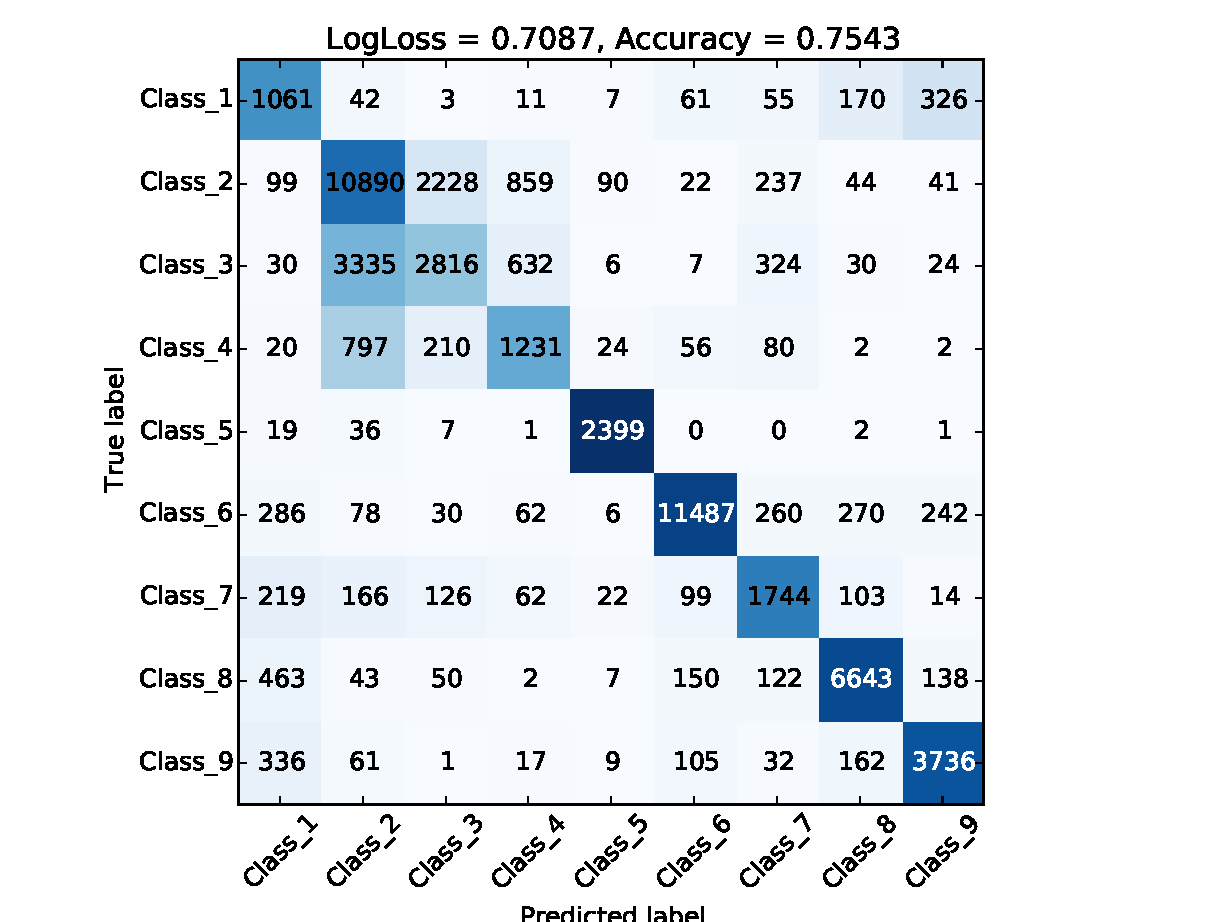
\includegraphics[width=0.7\textwidth]{LRcm_train}
	\caption{Logistic regression confusion matrix using training dataset}
	\label{fig:LRcm_train}
\end{figure}
\begin{figure}[h!]
	\centering
	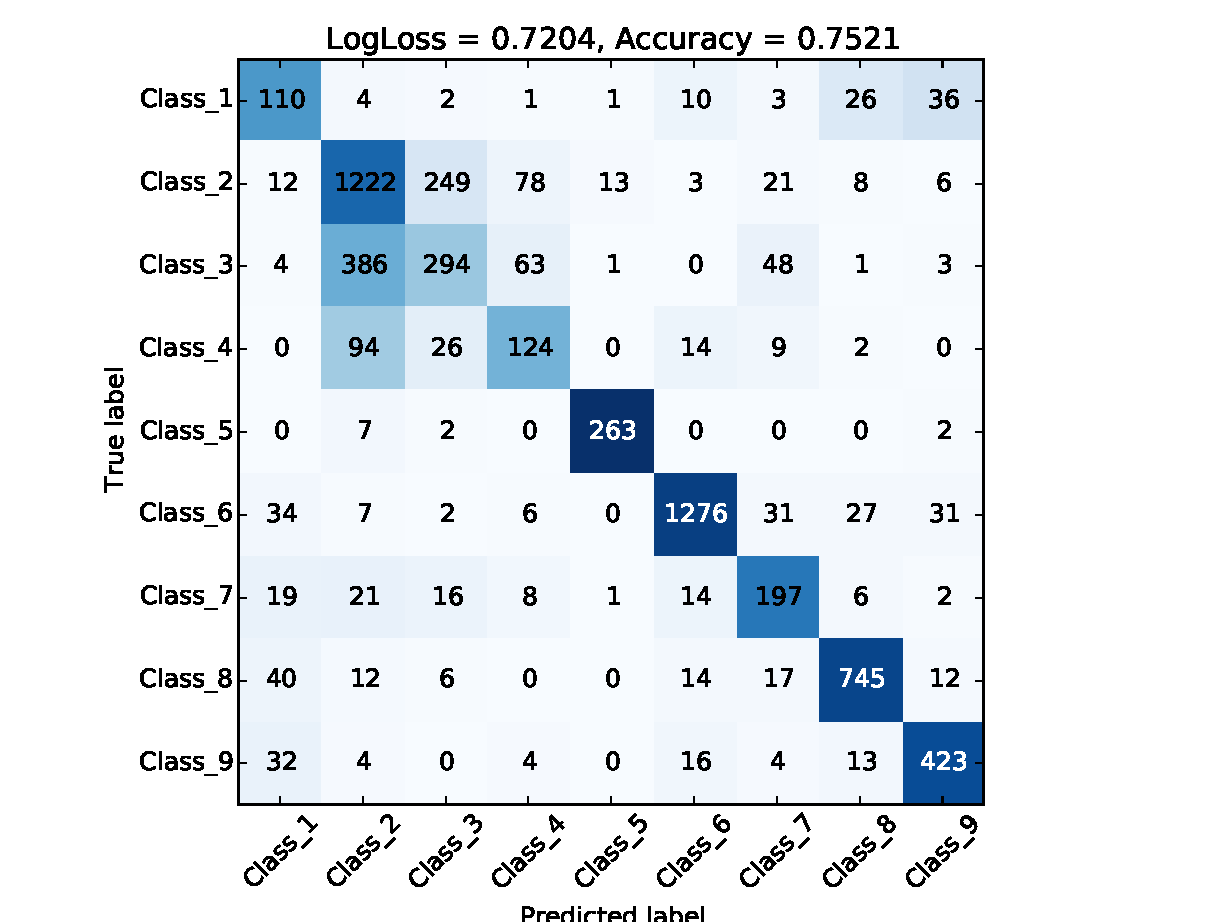
\includegraphics[width=0.7\textwidth]{LRcm_test}
	\caption{Logistic regression confusion matrix using testing dataset}
	\label{fig:LRcm_test}
\end{figure}
Performance using training and testing set is similar, but still not good enough. A lot of misclassifications are made among classes, specially between class 2 and 3.
\subsection{K-nearest neighbor}
\begin{table}[h!]
	\caption{The KNeighborsClassifier parameters}
	\begin{tabular}{ | l | l | p{7cm} |}
		\hline
		\textbf{Parameter} & \textbf{Default} & \textbf{Description}\\
		\hline
		$n\_neighbors$ & 5 & Number of neighbors to use.\\
		\hline
		$weights$ & uniform & weight function used in prediction.
		
		‘uniform’ : All points in each neighborhood are weighted equally. 
		
		‘distance’ : weight points by the inverse of their distance.\\
		\hline
		$algorithm$ & auto & Algorithm used to compute the nearest neighbors: ball\_tree, kd\_tree, brute (brute-force search) or auto. The last will attempt to decide the most appropriate algorithm based on the values passed to fit method.\\
		\hline
		$metric$ & minkowski & the distance metric to use for the tree.\\
		\hline
		$p$ & 2 & Power parameter for the Minkowski metric. When p = 1, this is equivalent to using manhattan\_distance, and euclidean\_distance for p = 2.\\
		\hline
	\end{tabular}
	\label{table:KNNdefaults}
\end{table}
The following set of hyper-parameter values was used:
\begin{itemize}
	\item n\_neighbors: [2, 3, 5, 7, 10, 15, 20]
	\item weights: ['uniform', 'distance']
	\item algorithm: ['ball\_tree', 'kd\_tree', 'brute']
	\item metric: ['minkowski']
	\item p: [1, 2, 3, 4, 5]
\end{itemize}
\subsubsection{Results}
\begin{table}[h!]
	\caption{Grid search output}
	\centering
	\begin{tabular}{ | l | c | c | c | c | c | c |}
		\hline
		$\bf{params_n}$ & \bf{n\_neighbors} & \bf{weights} & \bf{algorithm} & \bf{metric} & \bfseries{p}\  & \bfseries{log\_loss} \\ \hline
		$params_1$ & 20 & 'uniform' & 'brute' & 'minkowski' & 3 & 0.9871  \\ \hline
		$params_2$ & 20 & 'uniform' & 'kd\_tree' & 'minkowski' & 3 & 1.0305 \\ \hline
		$params_3$ & 15 & 'distance' & 'ball\_tree' & 'minkowski' & 3 & 1.0478 \\ \hline
		$params_4$ & 20 & 'uniform' & 'ball\_tree' & 'minkowski' & 5 & 1.1013 \\ \hline
		$params_5$ & 15 & 'distance' & 'ball\_tree' & 'minkowski' & 5 & 1.1176 \\ \hline
	\end{tabular}
\end{table}
%\vspace{2mm}
\begin{figure}[h!]
	\centering
	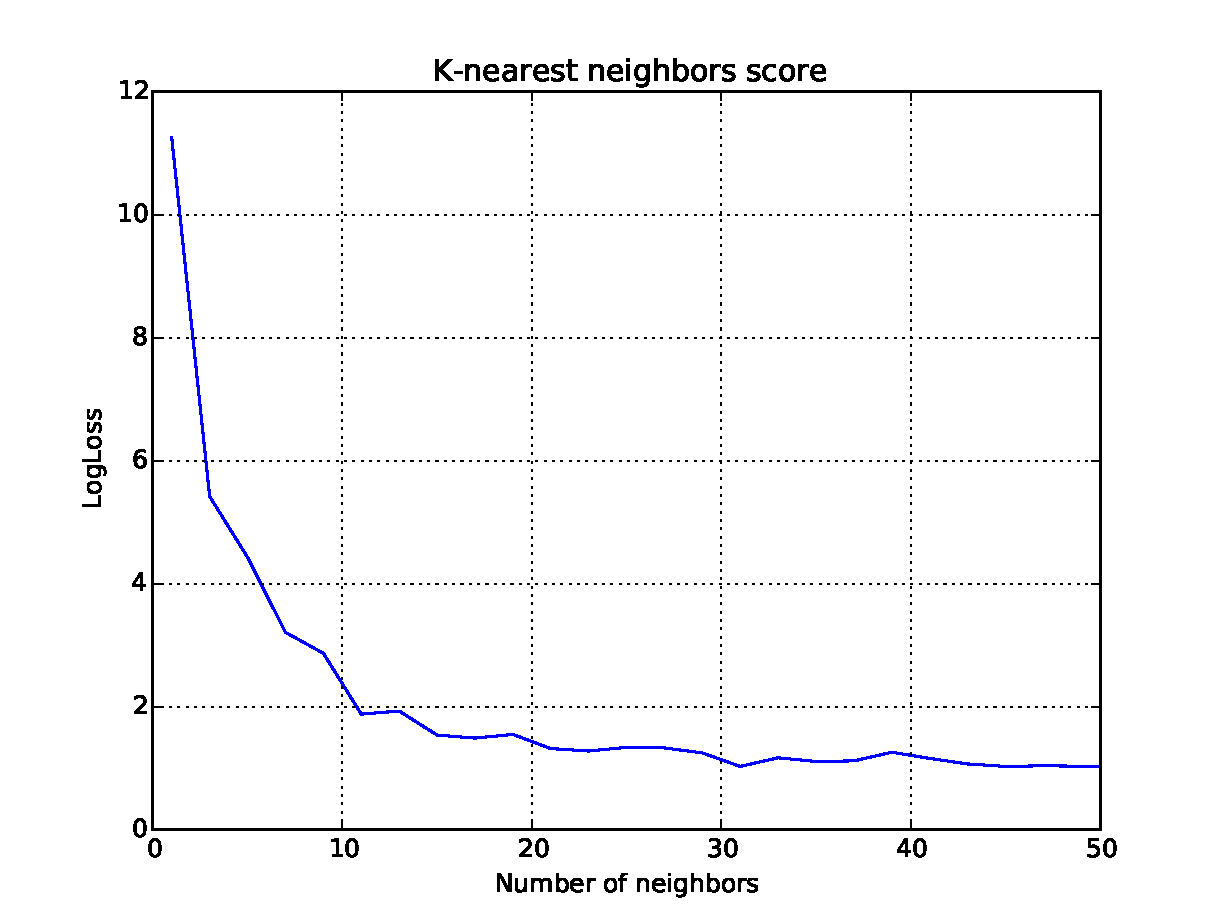
\includegraphics[width=0.8\textwidth]{KNN_scores}
	\caption{Scores varying the number of neighbors}
	\label{fig:KNN_scores}
\end{figure}
Figure \ref{fig:KNN_scores} was plotted by setting the $params_1$ obtained from the grid search and varying the number of neighbors. It can be appreciated that the LogLoss stops improving significantly passed the 30th neighbor.\\
\begin{figure}[h!]
	\centering
	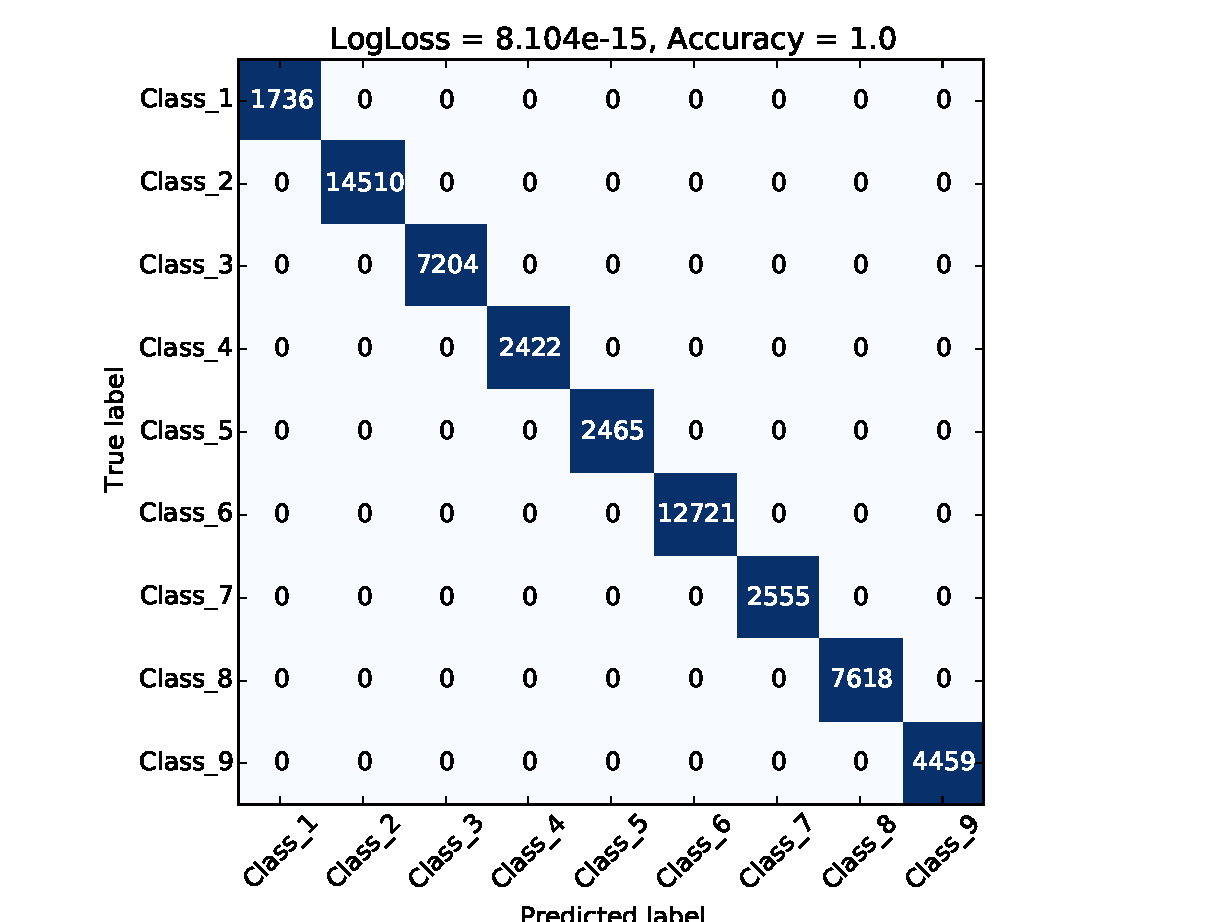
\includegraphics[width=0.7\textwidth]{KNNcm_train}
	\caption{k-NN confusion matrix using training dataset}
	\label{fig:KNNcm_train}
\end{figure}
\begin{figure}[h!]
	\centering
	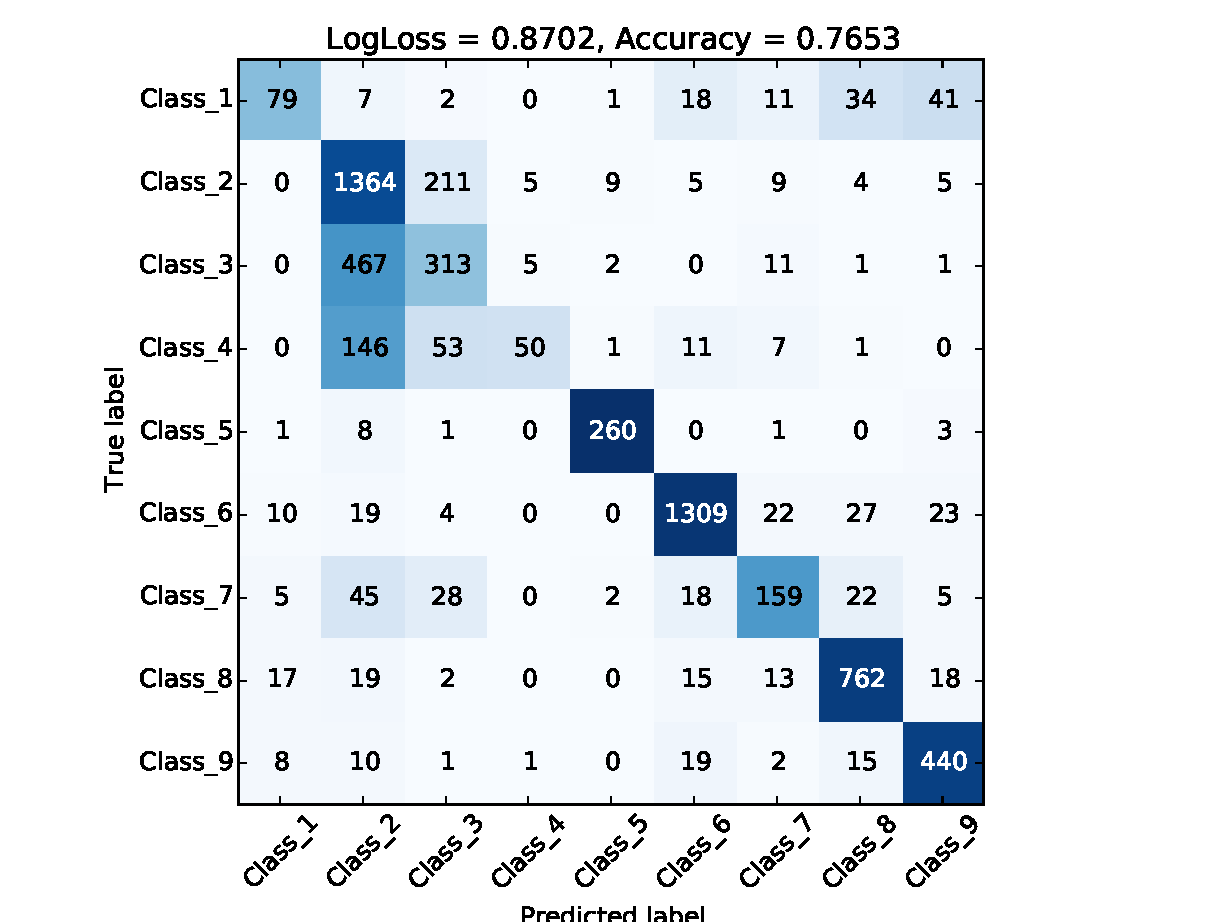
\includegraphics[width=0.7\textwidth]{KNNcm_test}
	\caption{k-NN confusion matrix using testing dataset}
	\label{fig:KNNcm_test}
\end{figure}\\
Because of the nature of the algorithm, measuring performance over the training set will always output a perfect accuracy because the points evaluated are exactly the same. The confusion matrix using the testing set gives us interesting results and an insight on how the data is arranged despite it's high dimensionality. There are lots of neighboring points between class 2, 3, and 4 which makes them the hardest classes to classify.\\
\subsection{Random Forests}
\begin{table}[h!]
	\caption{The RandomForestClassifier parameters}
	\begin{tabular}{ | l | l | p{7cm} |}
		\hline
		\textbf{Parameter} & \textbf{Default} & \textbf{Description}\\
		\hline
		$n\_estimators$ & 10 & Number of trees in the forest\\
		\hline
		$criterion$ & gini & Function to measure the quality of a split. "`gini"' for Gini impurity and "`entropy"' for information gain\\
		\hline
		$max\_depth$ & None &The maximum depth of the tree.\\
		\hline
		$max\_features$ & None & The number of features to consider when looking for the best split:\\
		\hline
	\end{tabular}
	\label{table:RFdefaults}
\end{table}
The following set of hyper-parameter values was used:\\
\begin{itemize}
	\item n\_estimators: 200
	\item criterion: ['gini', 'entropy']
	\item max\_depth: [2, 4, 6, 8],
	\item max\_features': [1.0, 0.7, 0.3, 0.1,'auto','sqrt','log2']
\end{itemize}
\subsubsection{Results}
\begin{table}[h!]
	\caption{Grid search output}
	\centering
	\begin{tabular}{ | l | c | c | c |}
		\hline
		$\bf{params_n}$ & \bf{criterion} &  \bf{mx\_features} & \bf{log\_loss} \\ \hline
		$params_1$ & 'gini' & 'auto' & 0.8646 \\ \hline
		$params_2$ & 'entropy' & 'auto' & 0.8969 \\ \hline
		$params_3$ & 'gini' & 'sqrt' & 0.9018 \\ \hline
		$params_4$ & 'gini' & 'log2' & 0.9336 \\ \hline
		$params_5$ & 'entropy' & 'log2' & 0.9635 \\ \hline
	\end{tabular}
\end{table}
The best parameters founds were selected, with exception of the number of estimators. This was varied in order to measure the performance vs the number of trees. It is important to remember that each tree in the forest is independent from one another and a large number of trees won't always imply that a better performance will be obtained even if testing over the training set.\\

Two different performance metrics were used, the LogLoss and the accuracy which as we can see in Figure \ref{fig:RFlog_loss} and Figure \ref{fig:RFaccuracy} behave differently. Accuracy is maintained relatively constant for both the training and testing set whereas the LogLoss provides us a more detailed visualization of the improvement in the predicted probabilities. Performance stops improving after 200 trees and no evident sign of overfitting is presented. If the only metric used was to be accuracy this fact couldn't be so easily seen leading to a less reliable score.\\
\begin{figure}[h!]
    \centering
    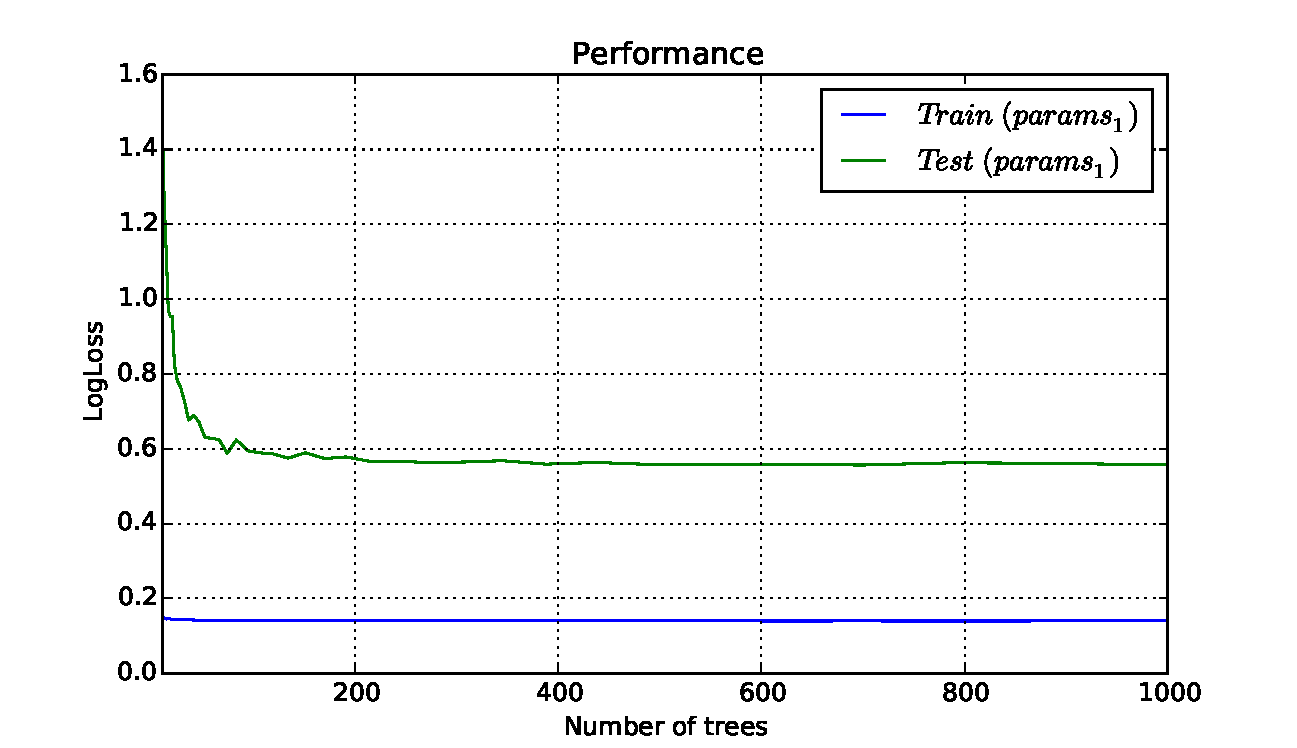
\includegraphics[width=1\textwidth]{RFlogloss}
    \caption{Performance using logarithmic loss as a metric}
    \label{fig:RFlog_loss}
\end{figure}\\
\begin{figure}[h!]
    \centering
    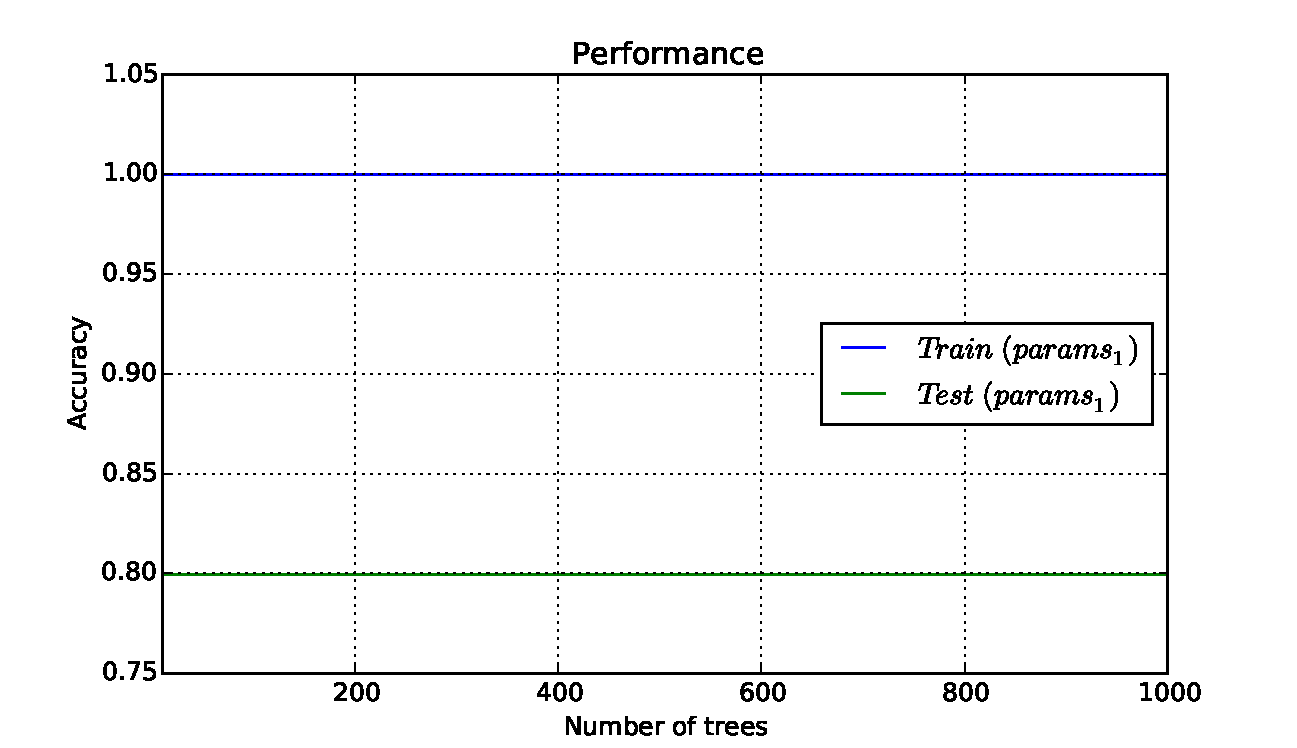
\includegraphics[width=1\textwidth]{RFaccuracy}
    \caption{Performance using accuracy as a metric}
    \label{fig:RFaccuracy}
\end{figure}\\
Confusion matrices were plotted using 400 as the number of estimators.
\begin{figure}[h!]
    \centering
    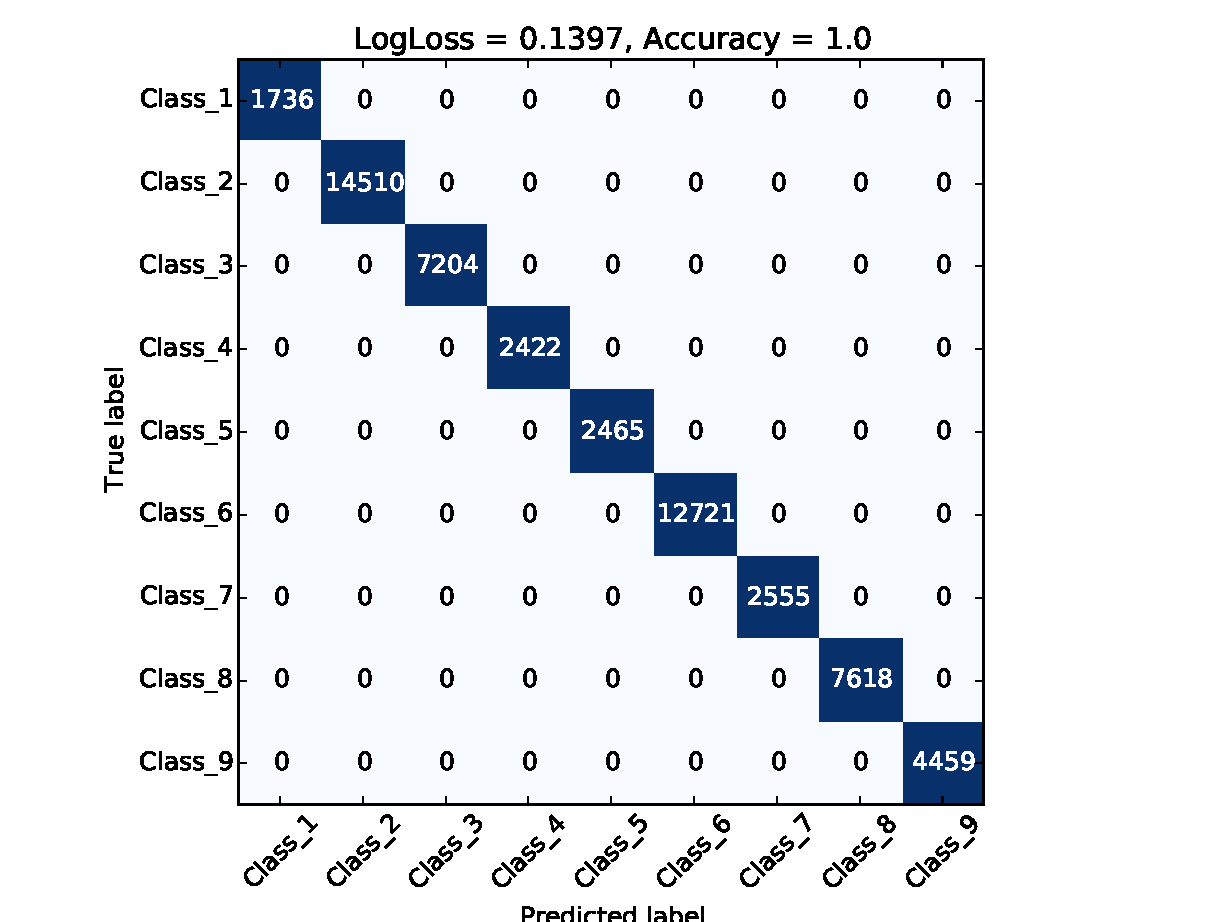
\includegraphics[width=0.7\textwidth]{RFcm_train}
    \caption{Random Forests confusion matrix using training dataset}
    \label{fig:RFcm_train}
\end{figure}
\begin{figure}[h!]
    \centering
    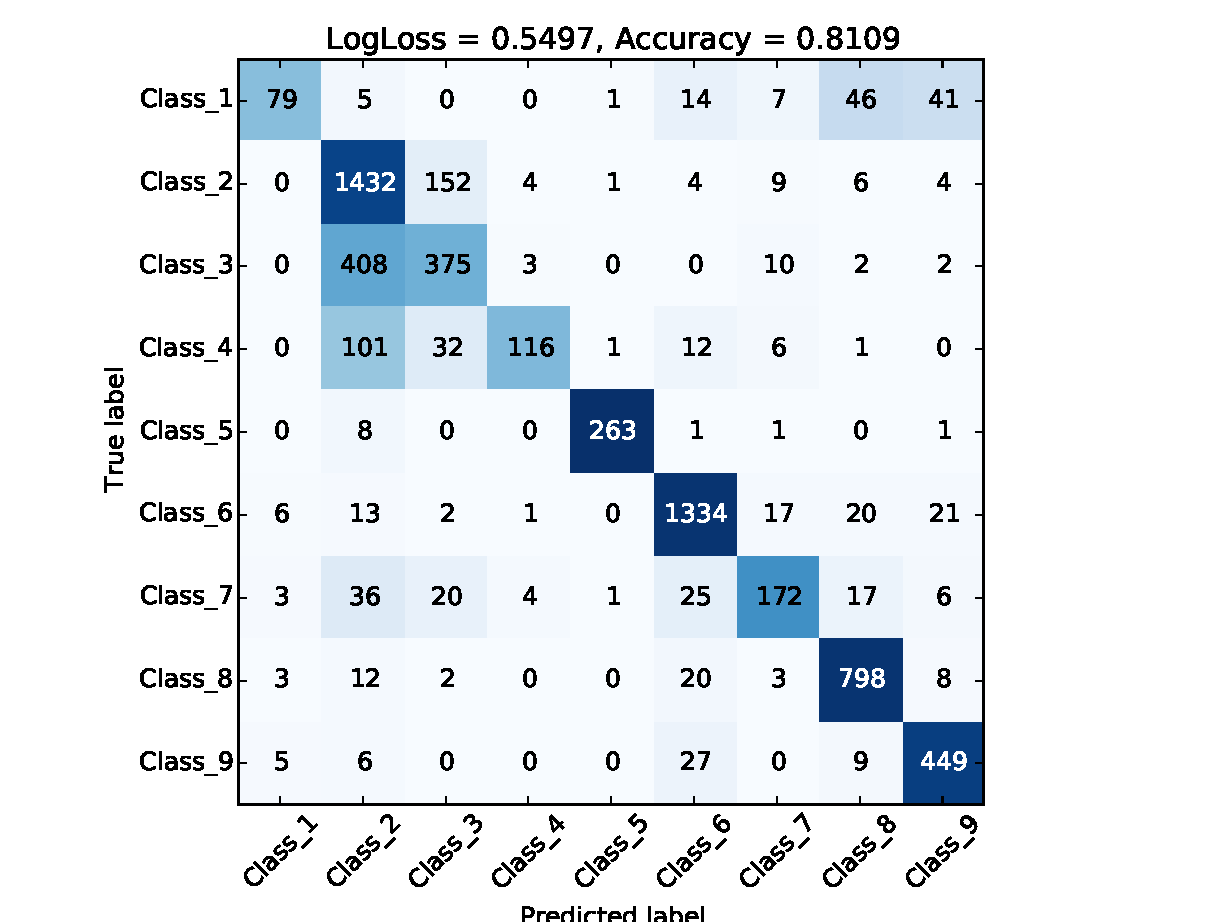
\includegraphics[width=0.7\textwidth]{RFcm_test}
    \caption{Random Forests confusion matrix using testing dataset}
    \label{fig:RFcm_test}
\end{figure}
\subsection{Gradient Boosting}
\begin{table}[h!]
	\caption{The GradientBoostingClassifier parameters}
	\begin{tabular}{ | l | l | p{7cm} |}
		\hline
		\textbf{Parameter} & \textbf{Default} & \textbf{Description}\\
		\hline
		$n\_estimators$ & 100 & The number of boosting stages to perform. Gradient boosting is fairly robust to over-fitting so a large number usually results in better performance.\\
		\hline
		$learning\_rate$ & 0.1 & learning rate shrinks the contribution of each tree by learning\_rate.\\
		\hline
		$max\_depth$ & 3 & The maximum depth limits the number of nodes in the tree.\\
		\hline
		$min\_samples\_leaf$ & 1 & The minimum number of samples required to be at a leaf node.\\
		\hline
		$max\_features$ & n\_features & The number of features to consider when looking for the best split.\\
		\hline
	\end{tabular}
	\label{table:GBdefaults}
\end{table}
The following set of hyper-parameter values was used:
\begin{itemize}
	\item learning\_rate: [0.1, 0.05, 0.02, 0.01],
	\item max\_depth: [2, 4, 6],
	\item min\_samples\_leaf: [3, 5, 9, 17],
	\item max\_features: [1.0, 0.7, 0.3, 0.1]
\end{itemize}
\subsubsection{Results}
\begin{table}[h!]
	\caption{Grid search output}
	\centering
	\begin{tabular}{ | l | c | c | c | c | c |}
		\hline
		$\bf{params_n}$ & \bf{l\_rate} &  \bf{mx\_depth} & \bf{m\_s\_leaf} & \bf{mx\_features} & \bf{log\_loss} \\ \hline
		$params_1$ & 0.05 & 4 & 17 & 0.7 & 0.6511 \\ \hline
		$params_2$ & 0.10 & 2 & 9 & 0.1 & 0.6756 \\ \hline
		$params_3$ & 0.05 & 4 & 17 & 0.1 & 0.7065 \\ \hline
		$params_4$ & 0.02 & 6 & 5 & 0.3 & 0.7143 \\ \hline
		$params_5$ & 0.05 & 4 & 5 & 0.3 & 0.7226 \\ \hline
	\end{tabular}
\end{table}
\begin{figure}[h!]
    \centering
    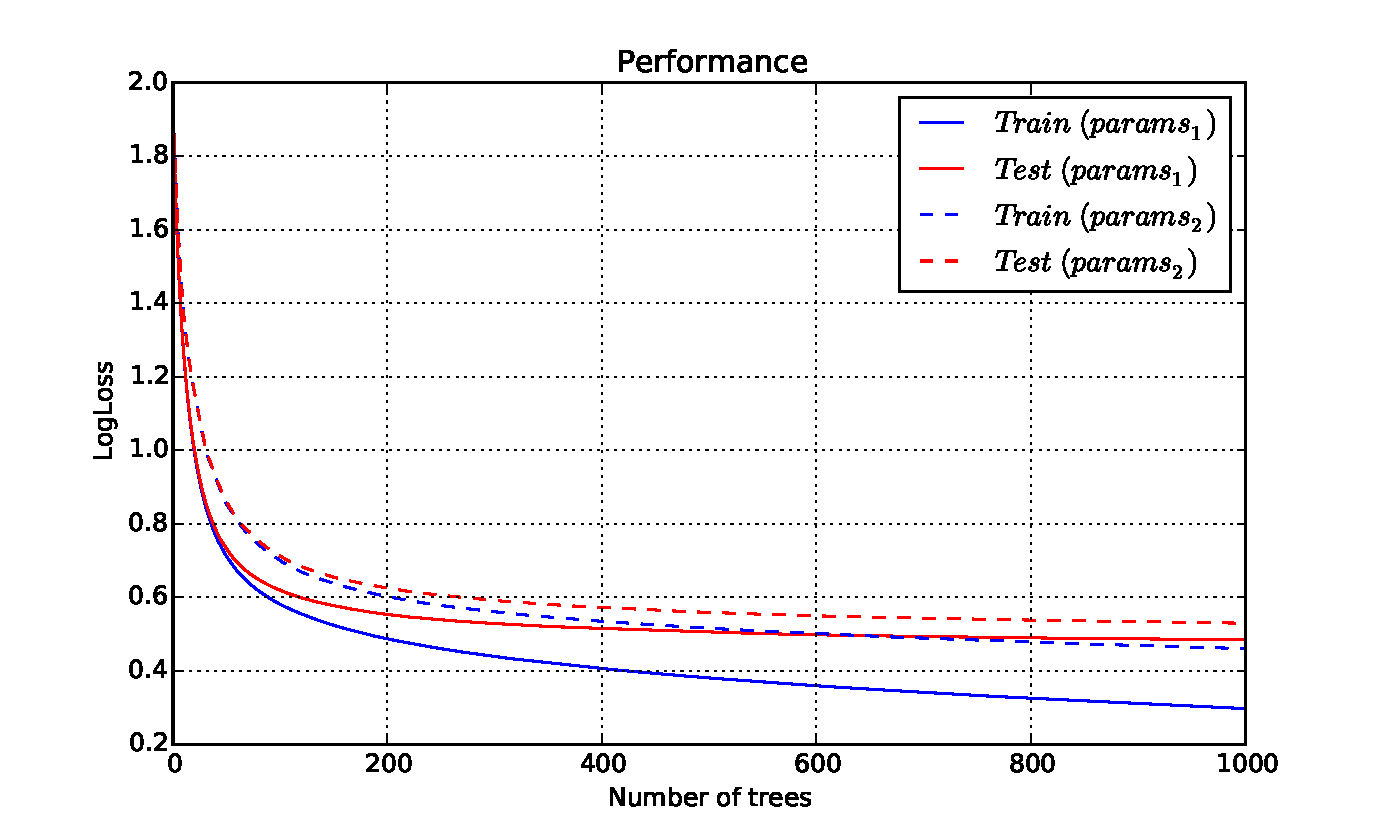
\includegraphics[width=0.86\textwidth]{GBlog_loss}
    \caption{Gradient boosting performance using logarithmic loss as a metric}
    \label{fig:GBlog_loss}
\end{figure}
\begin{figure}[h!]
    \centering
    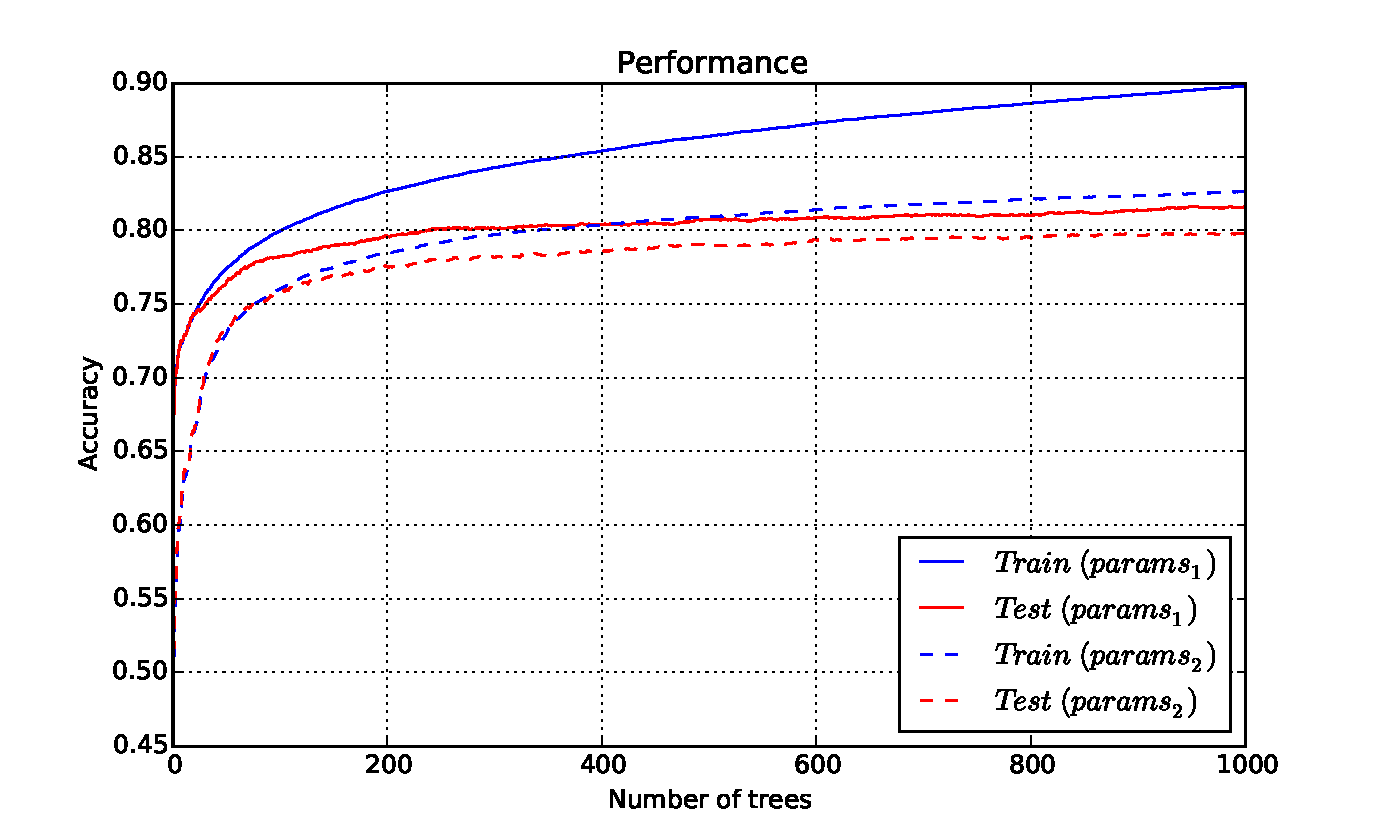
\includegraphics[width=0.9\textwidth]{GBaccuracy}
    \caption{Gradient boosting performance using accuracy as a metric}
    \label{fig:GBaccuracy}
\end{figure}
Knowing that, in boosting algorithms, each new classifier is an expert on the errors of its predecessor, we can compute the performance each time a new tree is added and plot it.

From figure \ref{fig:GBlog_loss} it can be seen that over-fitting is not present even with a large number of tree estimators. Differently from Random Forests, the accuracy changes with each tree that is added due to the fact that each new tree learns the errors of it's predecessor and a better output can be obtained. Performance improvement after the 500th tree is not significant and requires more memory and computation time.

\begin{figure}[h!]
    \centering
    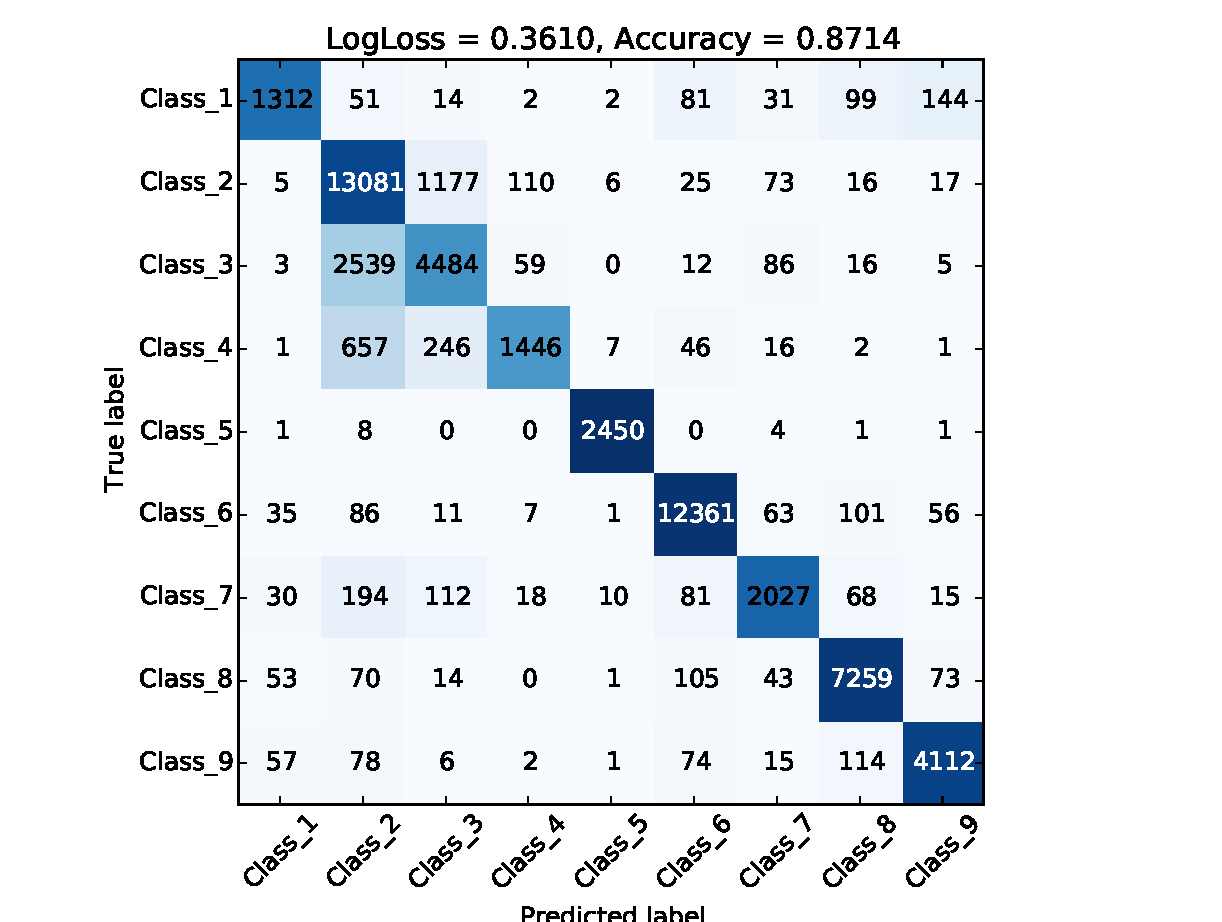
\includegraphics[width=0.69\textwidth]{GBcm_train}
    \caption{Gradient boosting confusion matrix using training set}
    \label{fig:GBcm_train}
\end{figure}
\begin{figure}[h!]
    \centering
    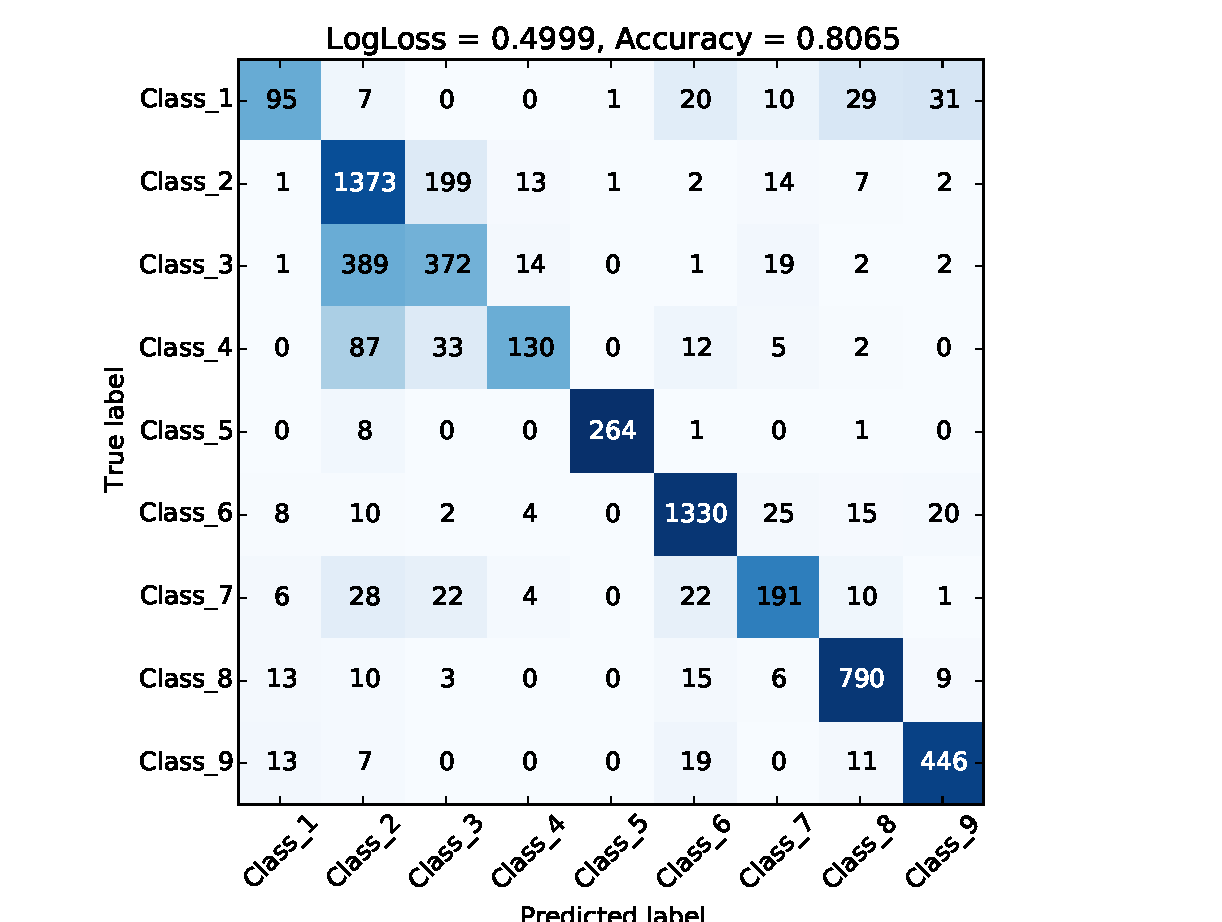
\includegraphics[width=0.7\textwidth]{GBcm_test}
    \caption{Gradient boosting confusion matrix using testing set}
    \label{fig:GBcm_test}
\end{figure}




\subsection{Combining predictions}
Having tested all the classifiers and obtaining ther respected probabilities we proceed to try to improve the overall performance by combining each of the predictions of the classifiers.

A brief summary can be visualized in Table \ref{table:summaryLogLoss}
\begin{table}[h!]
	\centering
	\caption{Test scores per classifier}
	\begin{tabular}{| l | c | c |}
		\hline
		\textbf{Classifier} & \textbf{Train} & \textbf{Test}\\
		\hline
		KNearestClassifier & 8.104e-15 & 0.8702 \\ \hline
		LogisticRegression & 0.7078 & 0.7204 \\ \hline
		RandomForestClassifier & 0.1397 & 0.5497 \\ \hline
		GradientBoostingClassifier & 0.3610 & 0.4978 \\ \hline
	\end{tabular}
	\label{table:summaryLogLoss}
\end{table}

From here we proceed to:
\begin{itemize}
	\item Average all 4 predictions
	\item Obtain weights to minimize LogLoss
\end{itemize}

From averaging predictions the final LogLoss is:

$$ LogLoss_{mean} = 0.5204 $$

Weights found after minimizing the LogLoss can be visualized in Figure \ref{fig:weights}
\begin{figure}[h!]
	\centering
	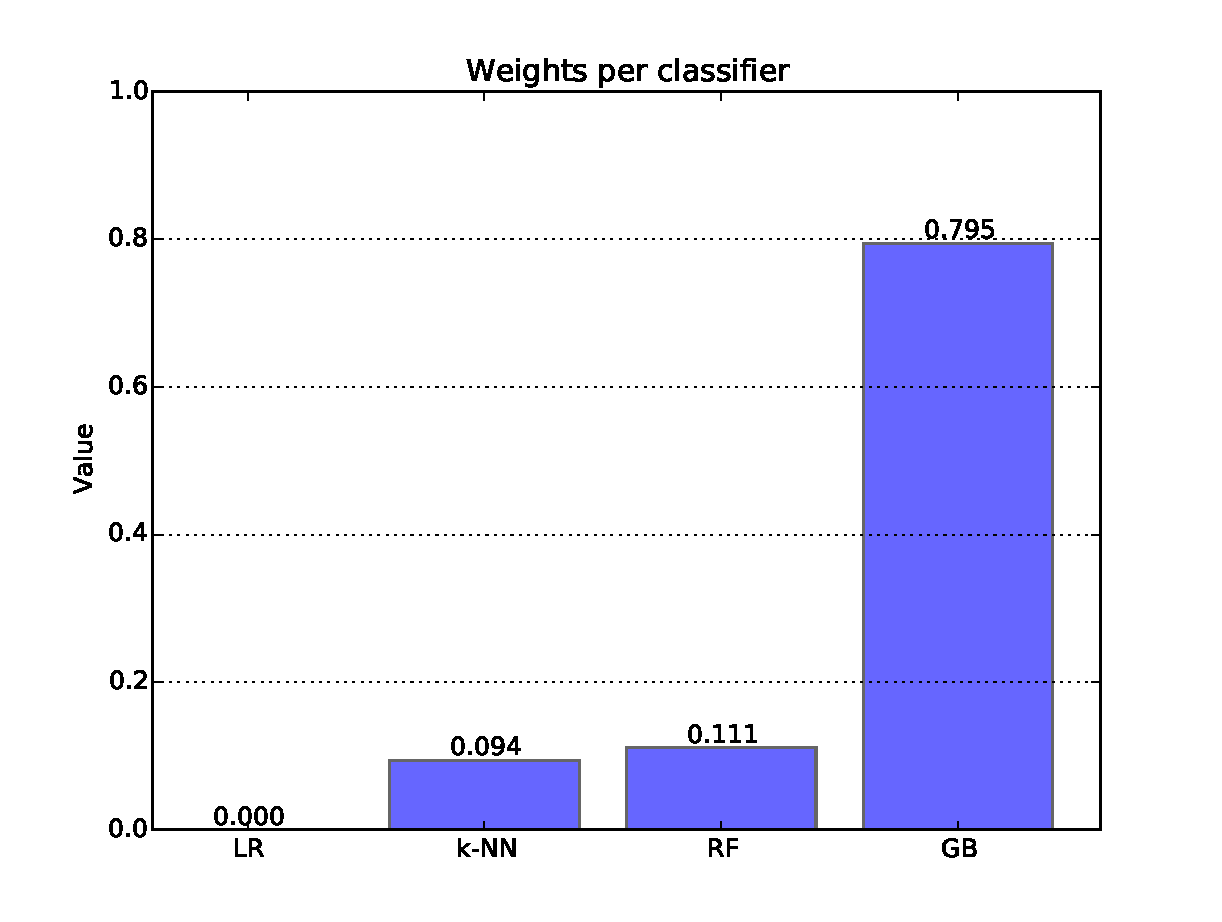
\includegraphics[width=0.8\textwidth]{weights}
	\caption{weights obtained from minimizing $LogLoss$ function}
	\label{fig:weights}
\end{figure}

$$ LogLoss_{weighted} = 0.4732 $$

The weights found can help ups identify which learning algorithms contribute the most to improving the LogLoss and which are practically useless. Indeed from Table \ref{table:summaryLogLoss} it can be foreseen that the output from Gradient Boosting would be one with most influence, however, even though the score using k-NN is the worst, it has nearly the same influence as Random Forest. Output obtained from Logistic Regression is practically useless given it's weight of $4.36e-7$.

\subsection{Computation time}
Even though no precise measurements for computation time in Table \ref{table:times} a general overview is presented where '$+++$' should be interpreted as 'fast' and '$---$' as 'slow'.

\begin{table}[h!]
	\centering
	\caption{Overview of training and predicting times}
	\begin{tabular}{| l | c | c |}
		\hline
		\textbf{Classifier} & \textbf{Training time} & \textbf{Predicting time}\\
		\hline
		KNearestClassifier & $+++$ & $---$ \\ \hline
		LogisticRegression & $++-$ & $++-$ \\ \hline
		RandomForestClassifier & $++-$ & $+--$ \\ \hline
		GradientBoostingClassifier & $+--$ & $++-$ \\ \hline
	\end{tabular}
	\label{table:times}
\end{table}

From the algorithms tested, the fastest to train is k-NN because it doesn't require training at all, and the slowest to train is gradient boosting. The fastest to predict is Logistic Regression followed by gradient boosting, and the slowest is k-NN because it has to make a search over all the dataset to find the k-nearest neighbors either by brute force or by some more efficient methods based on trees (ball tree or k-d tree).

It is interesting how both ensembles methods are inversely efficient, Random Forests is relatively fast to train but slow to predict and Gradient Boosting is the opposite. This is because in Random Forests th trees used are independent from each other with random samples from the data which makes training faster, however this trees have long depth which leads to a slow prediction. Gradient Boosting trees are connected and after the other making training slow, but the fact that this are weak learners (low depth trees) makes prediction faster. 